En esta sección se resolverán 2 problemas relacionados con \textit{string matching} usando el
algoritmo KMP y la función de error de la que se habló en el capítulo 4. Se resolverán los
problemas usando C++ y Haskell y se compararán ambas versiones.

%% TODO: Explicar los constraints

\section{SPOJ}
SPOJ (Sphere Online Judge)
% https://wiki.haskell.org/SPOJ
% Tomar algo del competitive aquí

\subsection{Encontrar el factor de repetición de una cadena}
Recordemos en el capítulo 3 \hyperlink{repetition_factor}{el problema 32.1}, es aquí cuando lo
bonito de la programación competitiva y resolver ejercicios se juntan. Ése problema es lo mismo
a resolver lo siguiente y aún mejor, en un juez en línea que puede ``probar'' la implementación.
La especificación del problema dice lo siguiente: 

% TODO: está dlv mi redacción, mejorarla.
Lo primero que se debe de hacer es calcular la función de error $\pi$ teniendo una complejidad en
tiempo de $\Theta(n)$ y lineal en espacio. Teniendo calculada $\pi$, consideremos $m$ la longitud
del patrón. Supongamos que $r = m - \pi[m]$ es la longitud de la $n$-esima raíz del patrón y que
$\pi[i] = i - r$ donde $r \mid m$ es la $\frac{i}{k}$-ésima concatenación de la raíz del patrón
hasta la $i$-ésima posición. Conlcuyendo así que $\rho(P) = \frac{m}{r}$.

En otro caso, supongamos que no se cumple lo anterior, i.e., que $r \nmid m$ entonces su factor de
repetición forzosamente debe ser 1. Por contradicción, supongamos que tiene un factor de repetición
mayor estrico que 1 lo que significaría que tendría que habría una cadena $x^r$ y que
$\pi[i] \geq \vert x^{r-1} \vert$, pero significaría que podríamos escribir a $x$ concatenada $r$
veces. $\Rightarrow\!\Leftarrow$

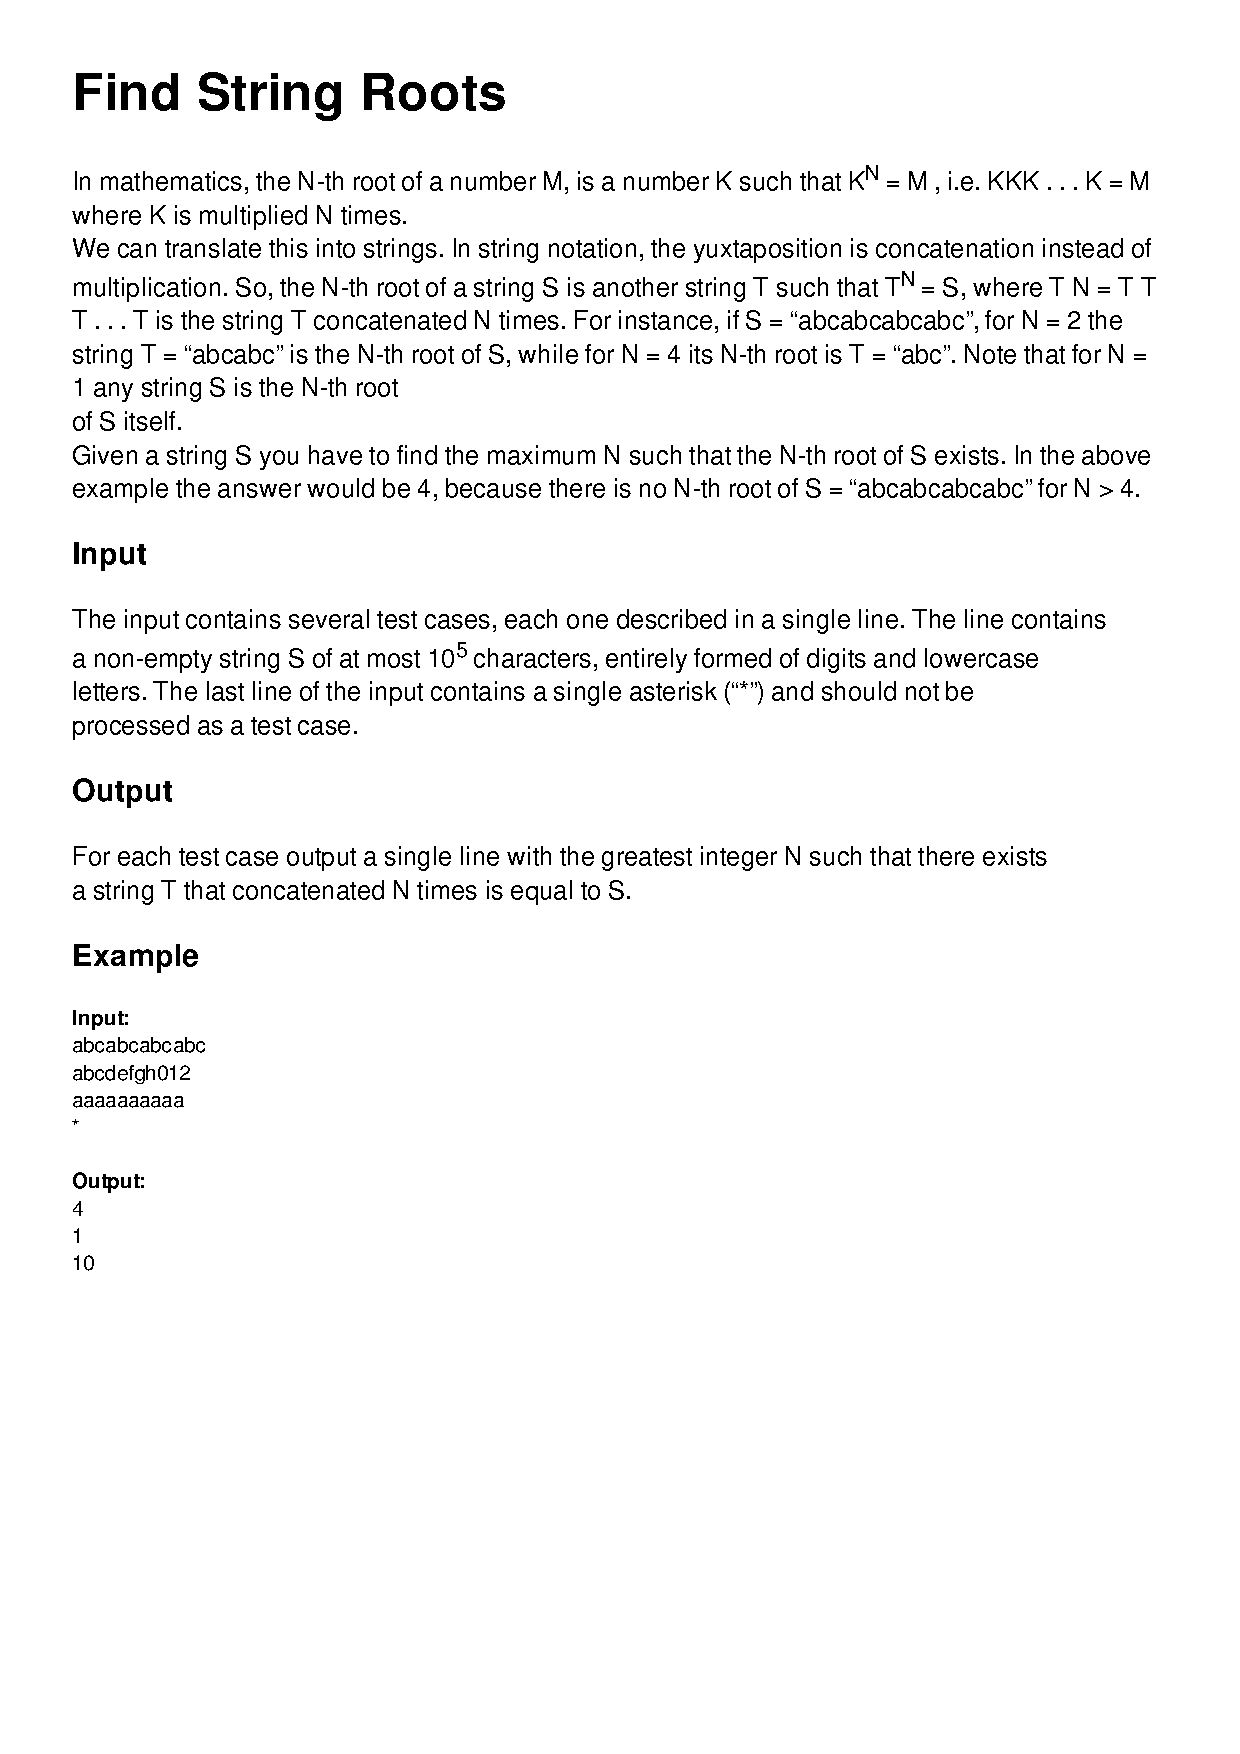
\includepdf[pages=-]{problemas/pdf/FINDSR.pdf}

\inputminted[linenos, frame=lines]{cpp}{problemas/cpp/FINDSR.cpp}
\pagebreak

En la línea 2 agregamos \texttt{vector} % TODO: explicar aquí qué pedo
De línea 6 a la 19 es la implementación de la función de error.
En la línea 23 es la parte importante sobre leer la entrada; una \textit{heurística} a seguir es que
siempre que diga: ``La entrada contiene varios casos de prueba, cada uno de ellos está descrito en una sola línea'', lo 
que se significa es que se seguirán leyendo valores de \texttt{cin} en la variable previamente declarada \texttt{x} simpre y cuando
el valor siga siendo leído se seguirá en el ciclo \texttt{while}.
% TODO: ecplicar que no nos fijamos en la cota de 10^5 caracteres
También menciona que la última entrada contendrá un solo asterisco \texttt{*} y es ahí cuando se parará de leer de la entrada estandar,
es por eso que primero se lee el valor y despué se compara que no sea diferente.

En la línea 24 se crea un vector cargado con la función de error con el patrón \texttt{s}.

La parte interesante aquí es en la línea 28 porque se obtiene la posible longitud de la $k$-ésima
raíz del patrón. Y de la línea 30 a 33 es cuando se hace la validación previamente analizada.

\inputminted[linenos, frame=lines]{haskell}{problemas/haskell/FINDSR.hs}
\pagebreak


En la línea 1 % TODO: explicar ahí qué pedoo

De la línea 19 a 29 es la implementación de función de error vista en el capítulo % TODO: poner vínculo al pendejo capótulo.

Analisemos parte por partes la línea 4, recordemos la función \\
\hsCode{interact :: (String -> String) -> IO ()} %% Ayudarme con lo de spoj

% TODO: está dlv mi redacción, mejorarla.
De la línea 9 a la 16 es la parte donde se hace el procesamiento del algoritmo principal,
en la expresión \hsCode{let ... in} % TODO: ver si así se podría poner
en la línea 10 se calcula la función de error de la cadena de entrada
en la línea 11 la función \hsCode{bounds :: Array i e -> (i, i)} devuelve los límites del arreglo en cual fue construido y nos quedamos
con la segunda entrada usando \hsCode{snd} para obtener el tamaño del arreglo.
En la línea 12 primero con la función \hsCode{(!) :: Ix i => Array i e -> i -> e} accedemos a la posición \texttt{m} del arreglo y recordando
la función \hsCode{ptable} la segunda entrada es el valor númerico del arreglo.
Acto seguido en la línea 13 oobtenemos  la posible longitud de la $k$-ésima
raíz del patrón. Y de la línea 14 a 15 es cuando se hace la validación previamente analizada.

% TODO: explicar los ejemplos del problema

\subsection{Ver si una cadena es una rotación cíclica de otra}
\hyperlink{cyclic_rotation}{el problema 32.4-7}
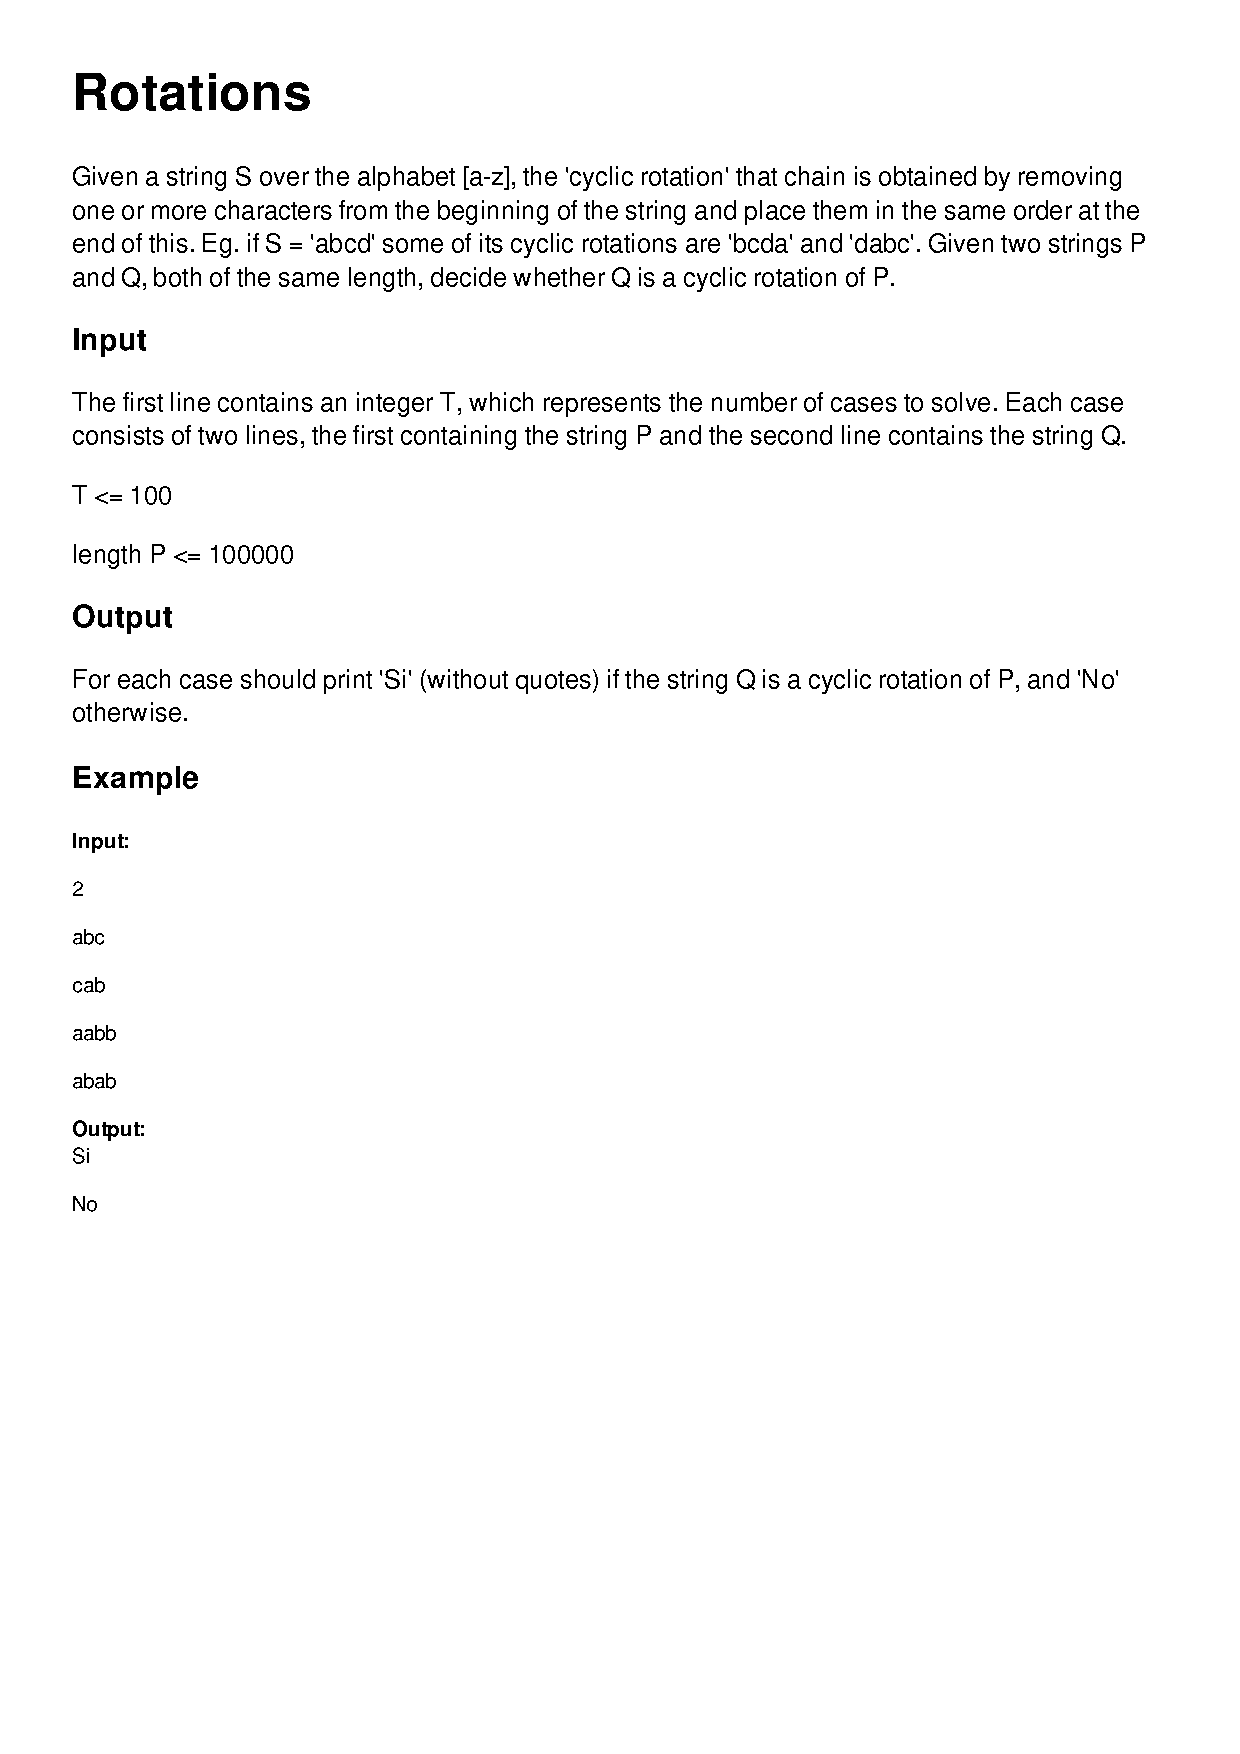
\includepdf[pages=-]{problemas/pdf/EC_WORLD.pdf}

\inputminted[linenos, frame=lines]{cpp}{problemas/cpp/EC_WORLD.cpp}
\pagebreak

\inputminted[linenos, frame=lines]{haskell}{problemas/haskell/EC_WORLD.hs}
\pagebreak

\subsection{Extender el palíndromo}
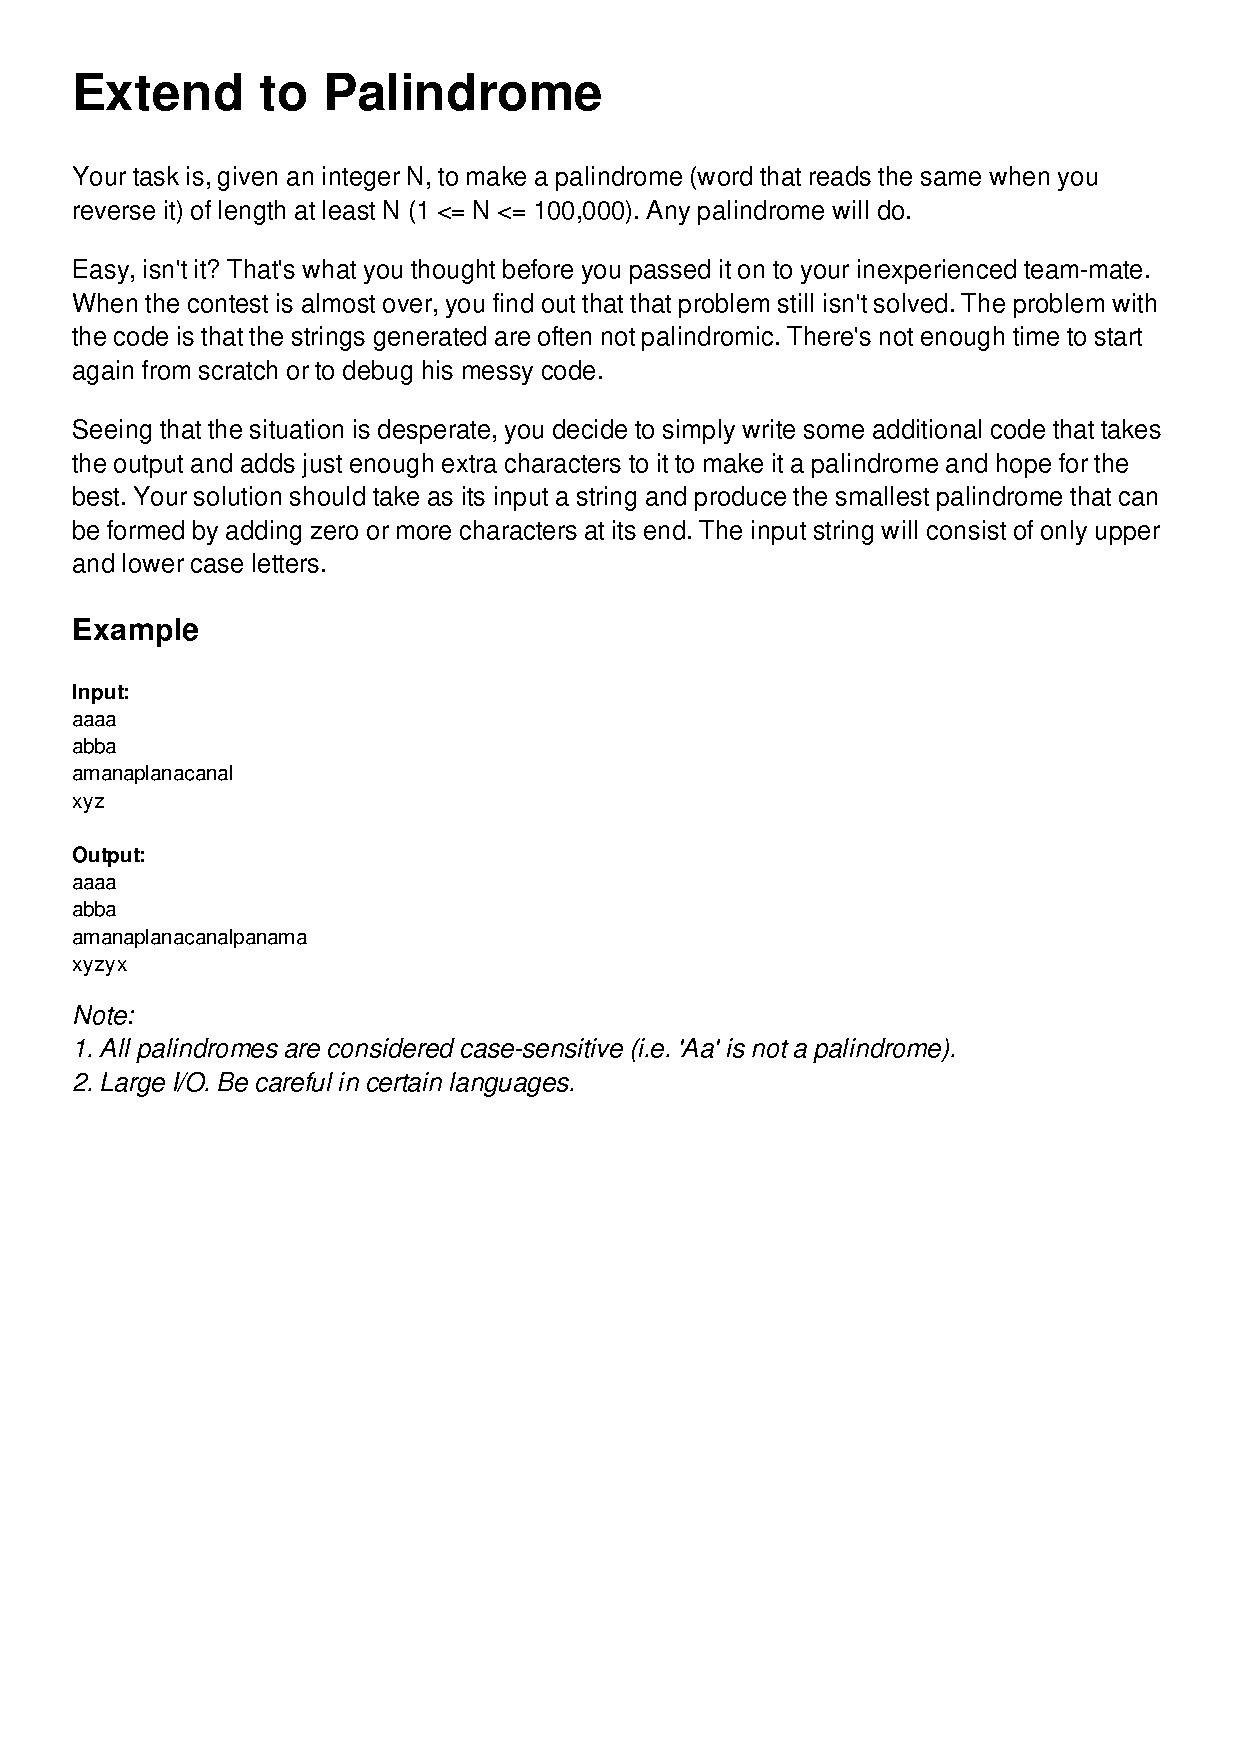
\includepdf[pages=-]{problemas/pdf/EPALIN.pdf}

\inputminted[linenos, frame=lines]{cpp}{problemas/cpp/EPALIN.cpp}
\pagebreak

\inputminted[linenos, frame=lines]{haskell}{problemas/haskell/EPALIN.hs}
\pagebreak

\subsection{Encontrar todas las ocurrencias de un patrón en un texto}
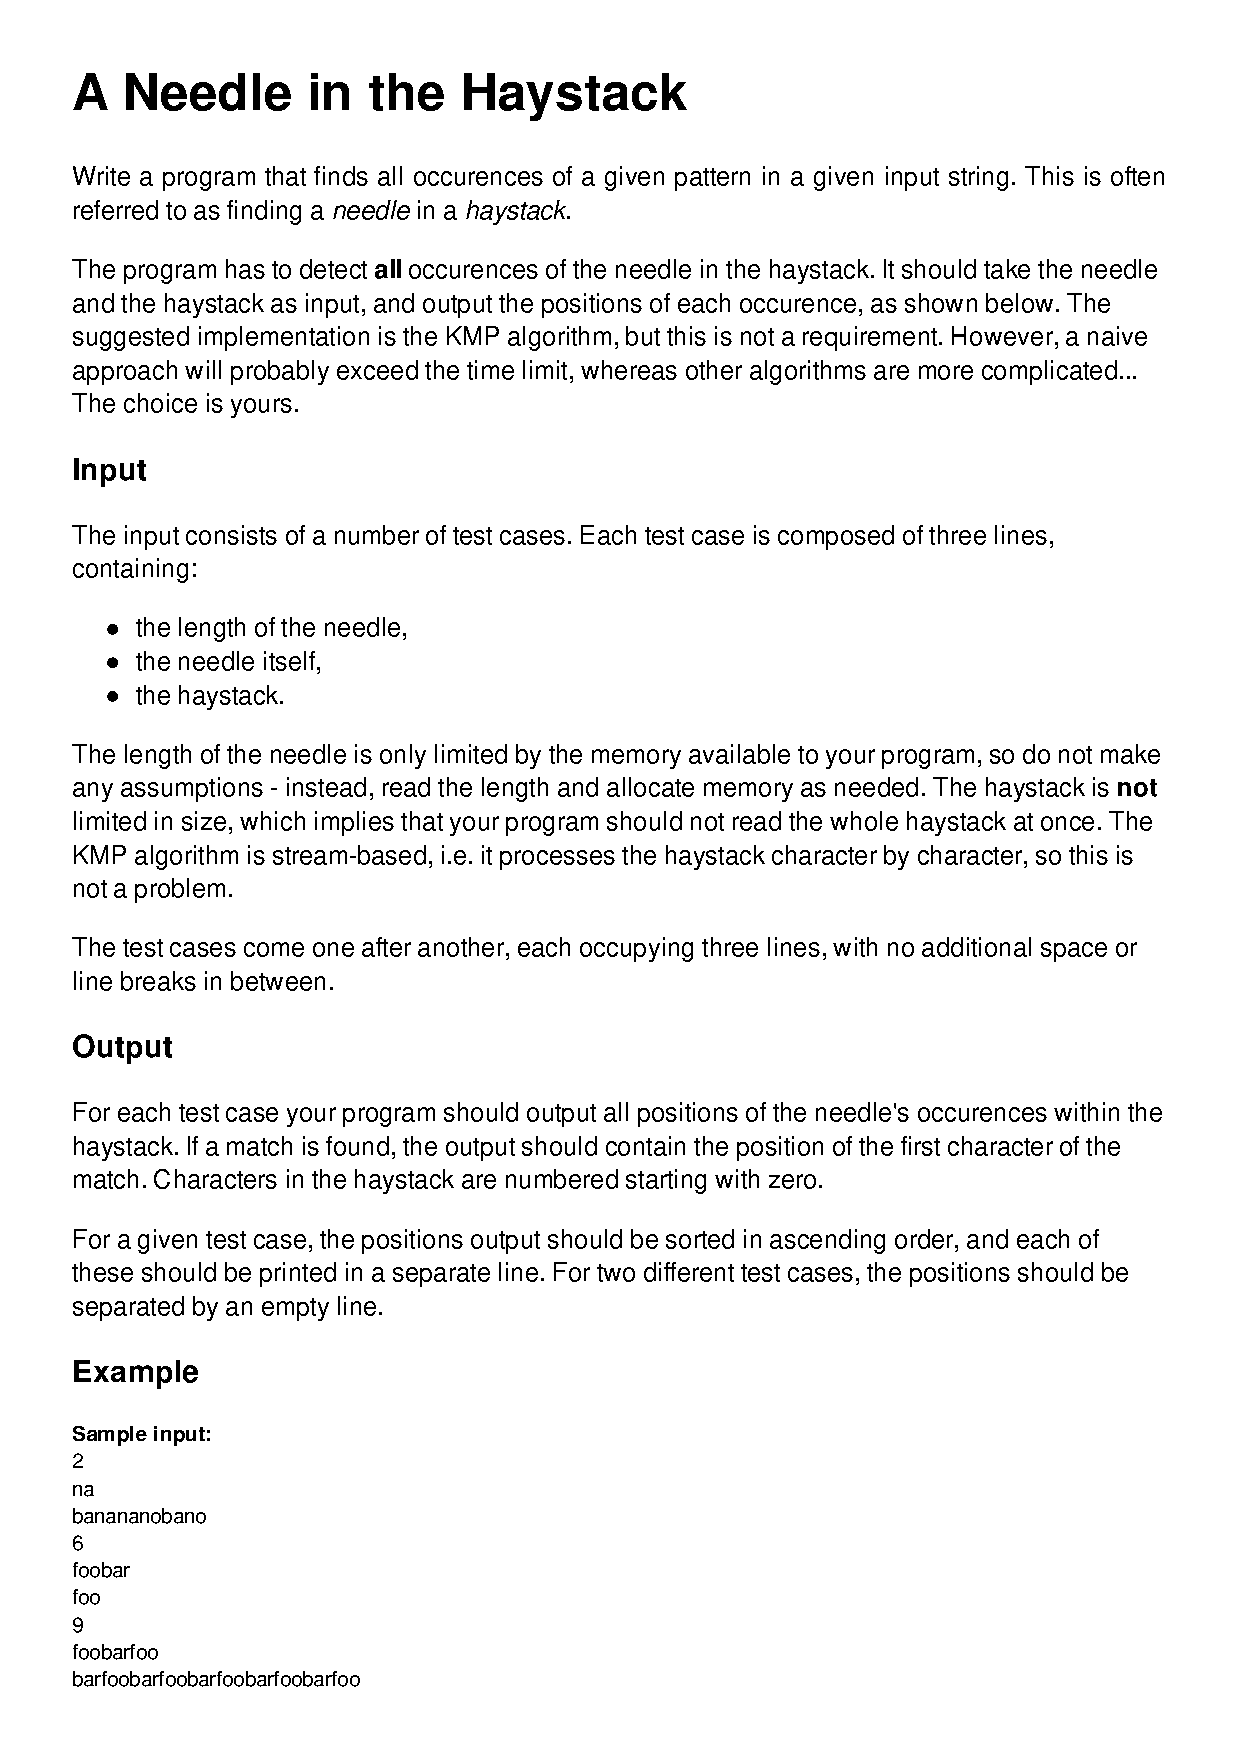
\includepdf[pages=-]{problemas/pdf/NHAY.pdf}

\inputminted[linenos, frame=lines]{cpp}{problemas/cpp/NHAY.cpp}
\pagebreak

\inputminted[linenos, frame=lines]{haskell}{problemas/haskell/NHAY.hs}
\pagebreak

% TODO: Chane y justifico esto el <$> https://ro-che.info/articles/2019-07-22-associativity-of-fmap

